\documentclass{a0poster}

\usepackage{fancytikzposter}
\usepackage{tikz}
\usepackage{xcolor}
\usepackage{titlesec}
\usepackage{array}
\usepackage[slovak]{babel}
\usepackage[utf8]{inputenc}
\usepackage[IL2]{fontenc}
\usepackage[utf8]{inputenc}
\usepackage{wrapfig}
\usepackage{xspace}
\usepackage{graphicx}       % vkládání obrázků





\usetikzlibrary{positioning, shapes, trees, graphs} % RNA trees
\usetikzlibrary{decorations.pathmorphing} % noisy shapes
\usetikzlibrary{fit}					% fitting shapes to coordinates
\usetikzlibrary{backgrounds}	% drawing the background after the foreground

\usepackage[pdftex,unicode]{hyperref}   % Musí být za všemi ostatními balíčky

\def\email{\href{mailto:richard.elias@matfyz.cz}{\nolinkurl{richard.elias@matfyz.cz}}}
\def\web{\href{http://richard.elias.matfyz.cz}{\nolinkurl{richard.elias.matfyz.cz}}}
\def\Autor{Richard Eliáš}
\def\Fakulta{Matematicko-fyzikální fakulta}
\def\Nazov{Vizualizace sekundární struktury RNA s využitím existujících struktur}

\newcommand{\Cdel}{\ensuremath{c_{del}}\xspace}
\newcommand{\Cins}{\ensuremath{c_{ins}}\xspace}
\newcommand{\Cupd}{\ensuremath{c_{upd}}\xspace}

\hypersetup{breaklinks=true}
\hypersetup{pdftitle={\Nazov}}
\hypersetup{pdfauthor={\Autor}}
\hypersetup{urlcolor=blue}


\renewcommand{\baselinestretch}{1.25} %riadkovanie
\renewcommand{\BackgroundPicture}[0]{
  \tikz[remember picture,overlay,opacity=.3]{
      \node at(current page.center){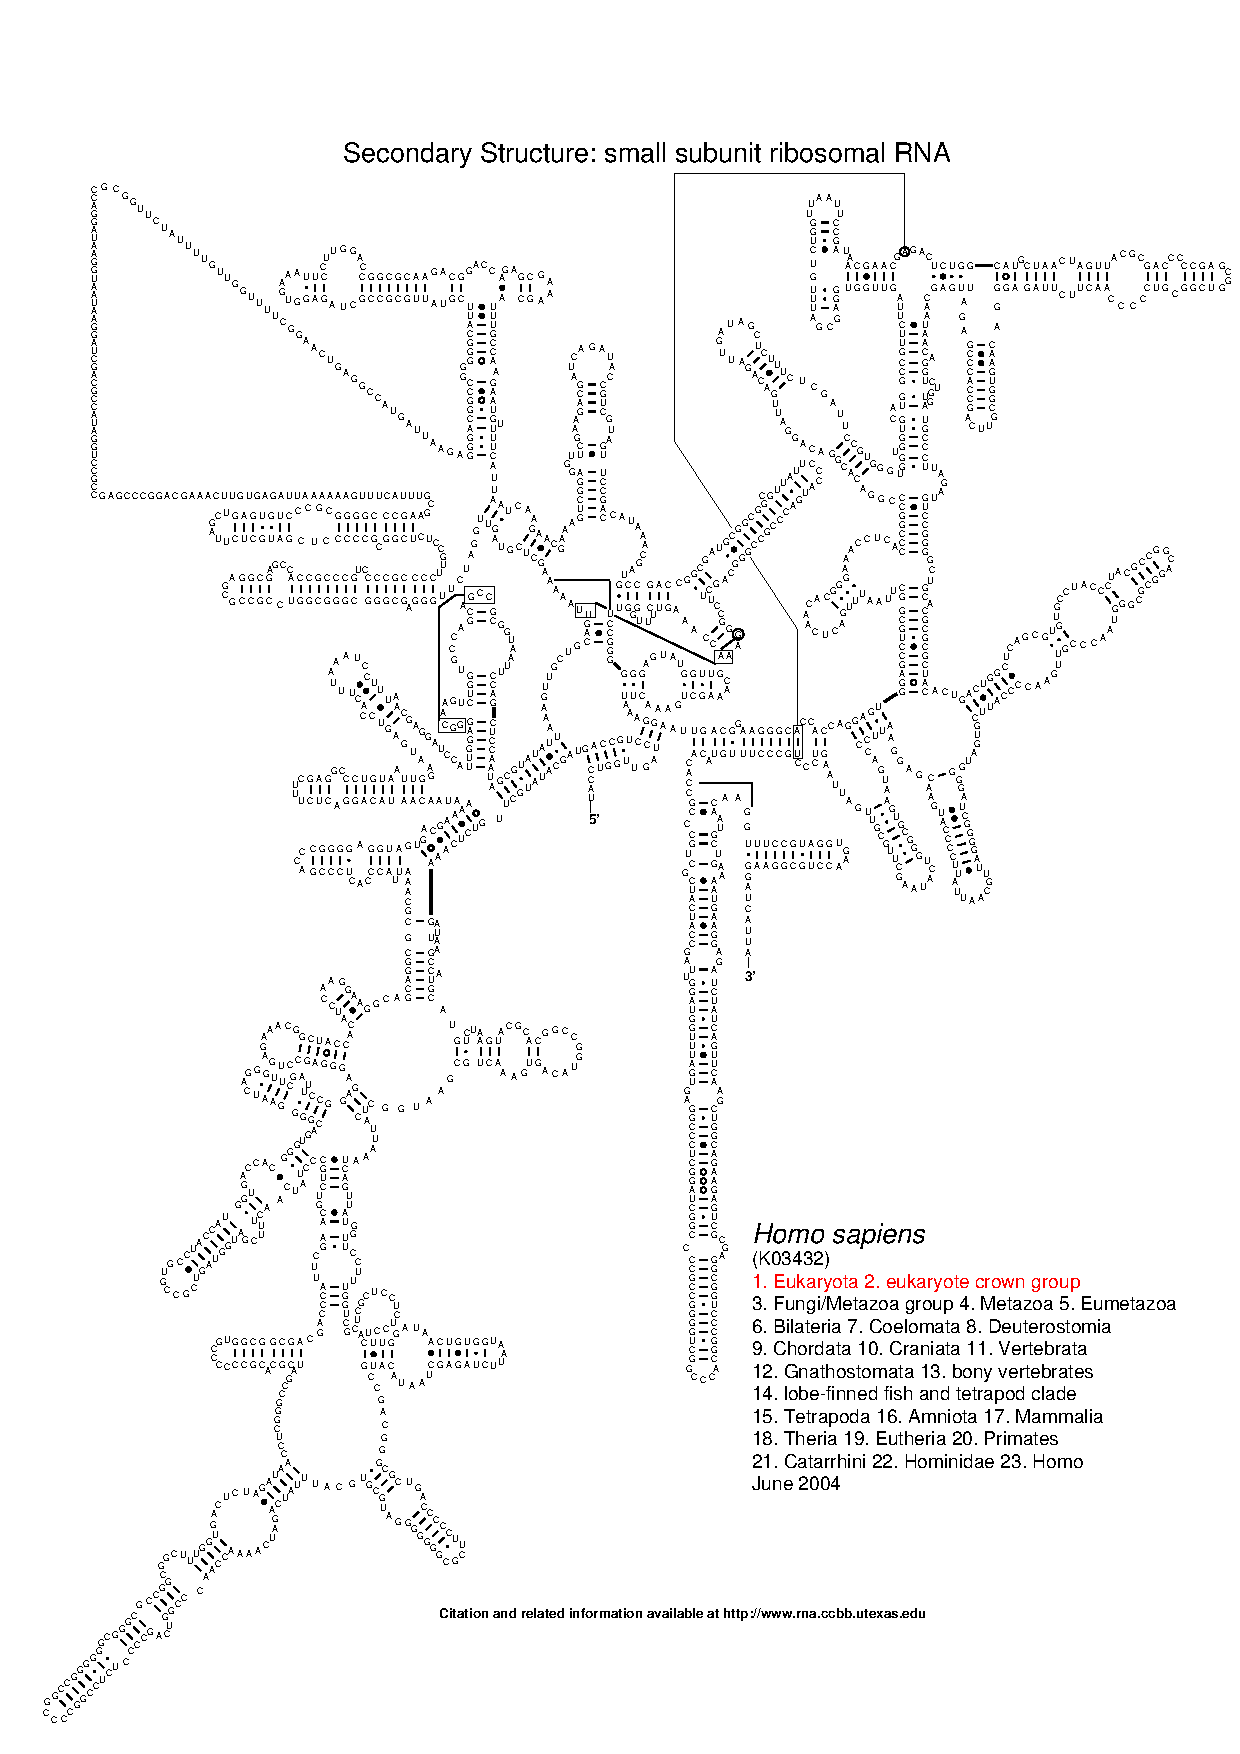
\includegraphics[height=\textheight]{../../text/img/human_crw.pdf}};
    }
  }



\title{\Nazov}
\author{\Autor\\\Fakulta\\\texttt{\email}}
\begin{document}
\AddToShipoutPicture{\BackgroundPicture}
\noindent
\begin{tikzpicture}
  \initializesizeandshifts
  \titleblock{50}{1}
  \blocknode{Motivácia a ciele práce}{
    Molekula RNA sa stáva predmetom mnohých štúdií, vďaka čomu rastie
    dopyt po nástrojoch pomáhajúcich pri jej analýze. Vlastnosti molekuly
    sú síce ovplyvnené primárou štruktúrou (poradím nukleotidov v~reťazci),
    no viac závisia na ich priestorovom usporiadaní (terciárna štruktára).
    My sa v~práci zaoberáme trochu zjednodušeným modelom - sekundárnou
    štruktúrou. Tú reprezentuje zoznam nukleotidov spojených väzbou.
    Tieto nukleotidy musia byť blízko aj v~priestore a~tak nám sekundárna štruktúra
    relatívne dobre aproximuje terciárnu, pre ktorú neexistujú spoľahlivé
    metódy zisťovania štruktúry už ani pre relatívne malé molekuly.

    Prvým krokom pri analýze RNA molekuly je často rozbor obrázka jej sekundárnej
    štruktúry. Medzi základné kritéria ktoré musia obrázky molekúl spľňať
    patrí rovinnosť nakreslenia, kreslenie loopov na kružnice a~stemy na priamkách.
    Pri porovnávaní štruktúr sa využíva taktiež kreslenie častí majúcich podobnú
    funkciu a~tvar na rovnaké miesta v~obrázkoch, čo pomáha lepšej orientácií
    v~molekule a~napomáha nájsť konzervované časti v~molekulách.
    V súčastných nástrojoch (mFold, RNAViz, RNAView, $\cdots$) sa toto posledné
    kritérium nedodržuje, čo má za následok ťažké nachádzanie konzervovaných častí
    v molekulách.
  }

  \blocknode{Kreslenie chýbajúcich častí v molekule}{XYZ}
  \blocknode{Obrazky, grafy, statistika}{\innerblock{Graf1}{XYZ\\ABC}}

  \startsecondcolumn
  \blocknode{Stromová reprezentácia RNA a použitie tree-edit-distance algoritmu}{
    \begin{wrapfigure}{L}{0.35\textwidth}
      \begin{tikzpicture}[
          on grid,
          node distance = 10cm,
          every node/.style = {rectangle, fill = none, draw = none}]
          \node (tree) {
            %trim=left bottom right top
            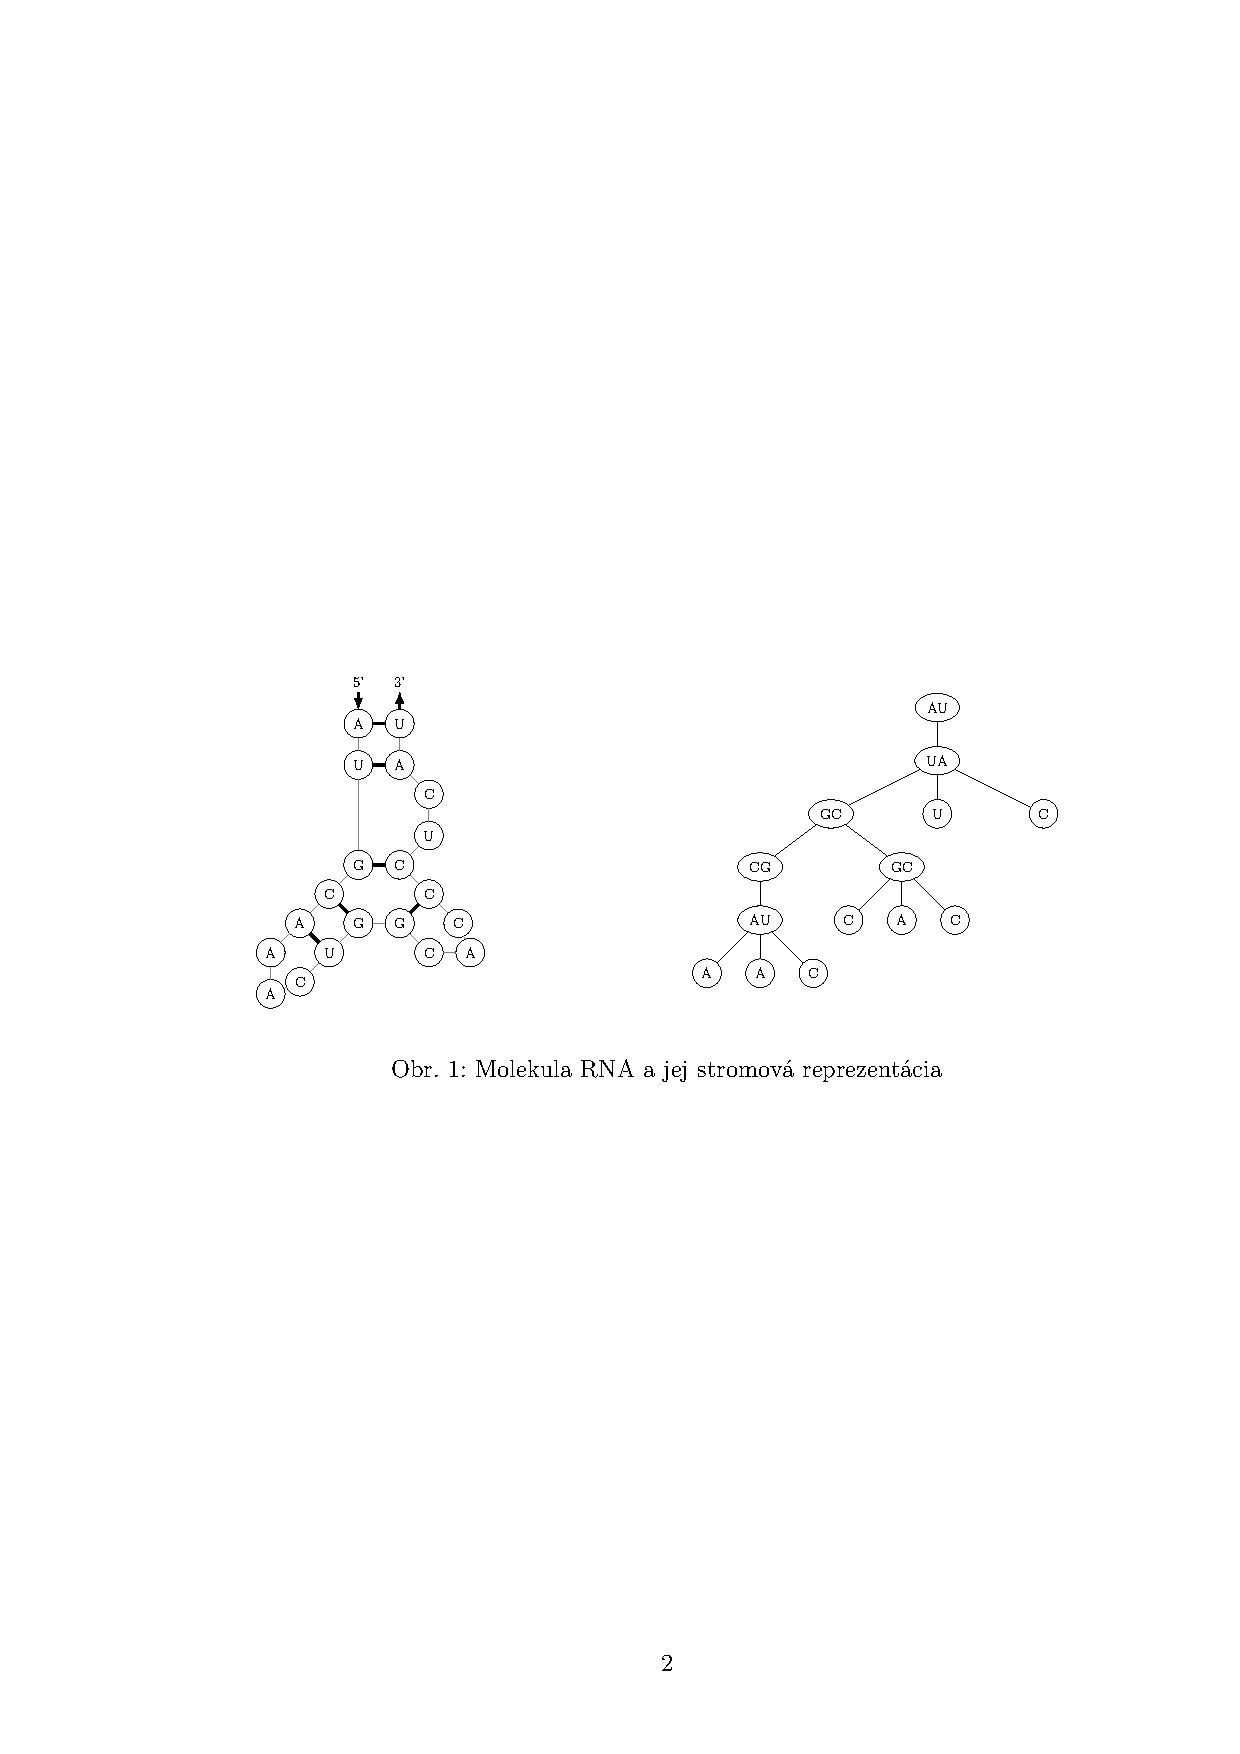
\includegraphics[clip, trim = 4cm 12cm 3cm 11cm, width=0.3\textwidth]{./include/rna_tree}
          };
          \node [below = of tree]{
            %trim=left bottom right top
            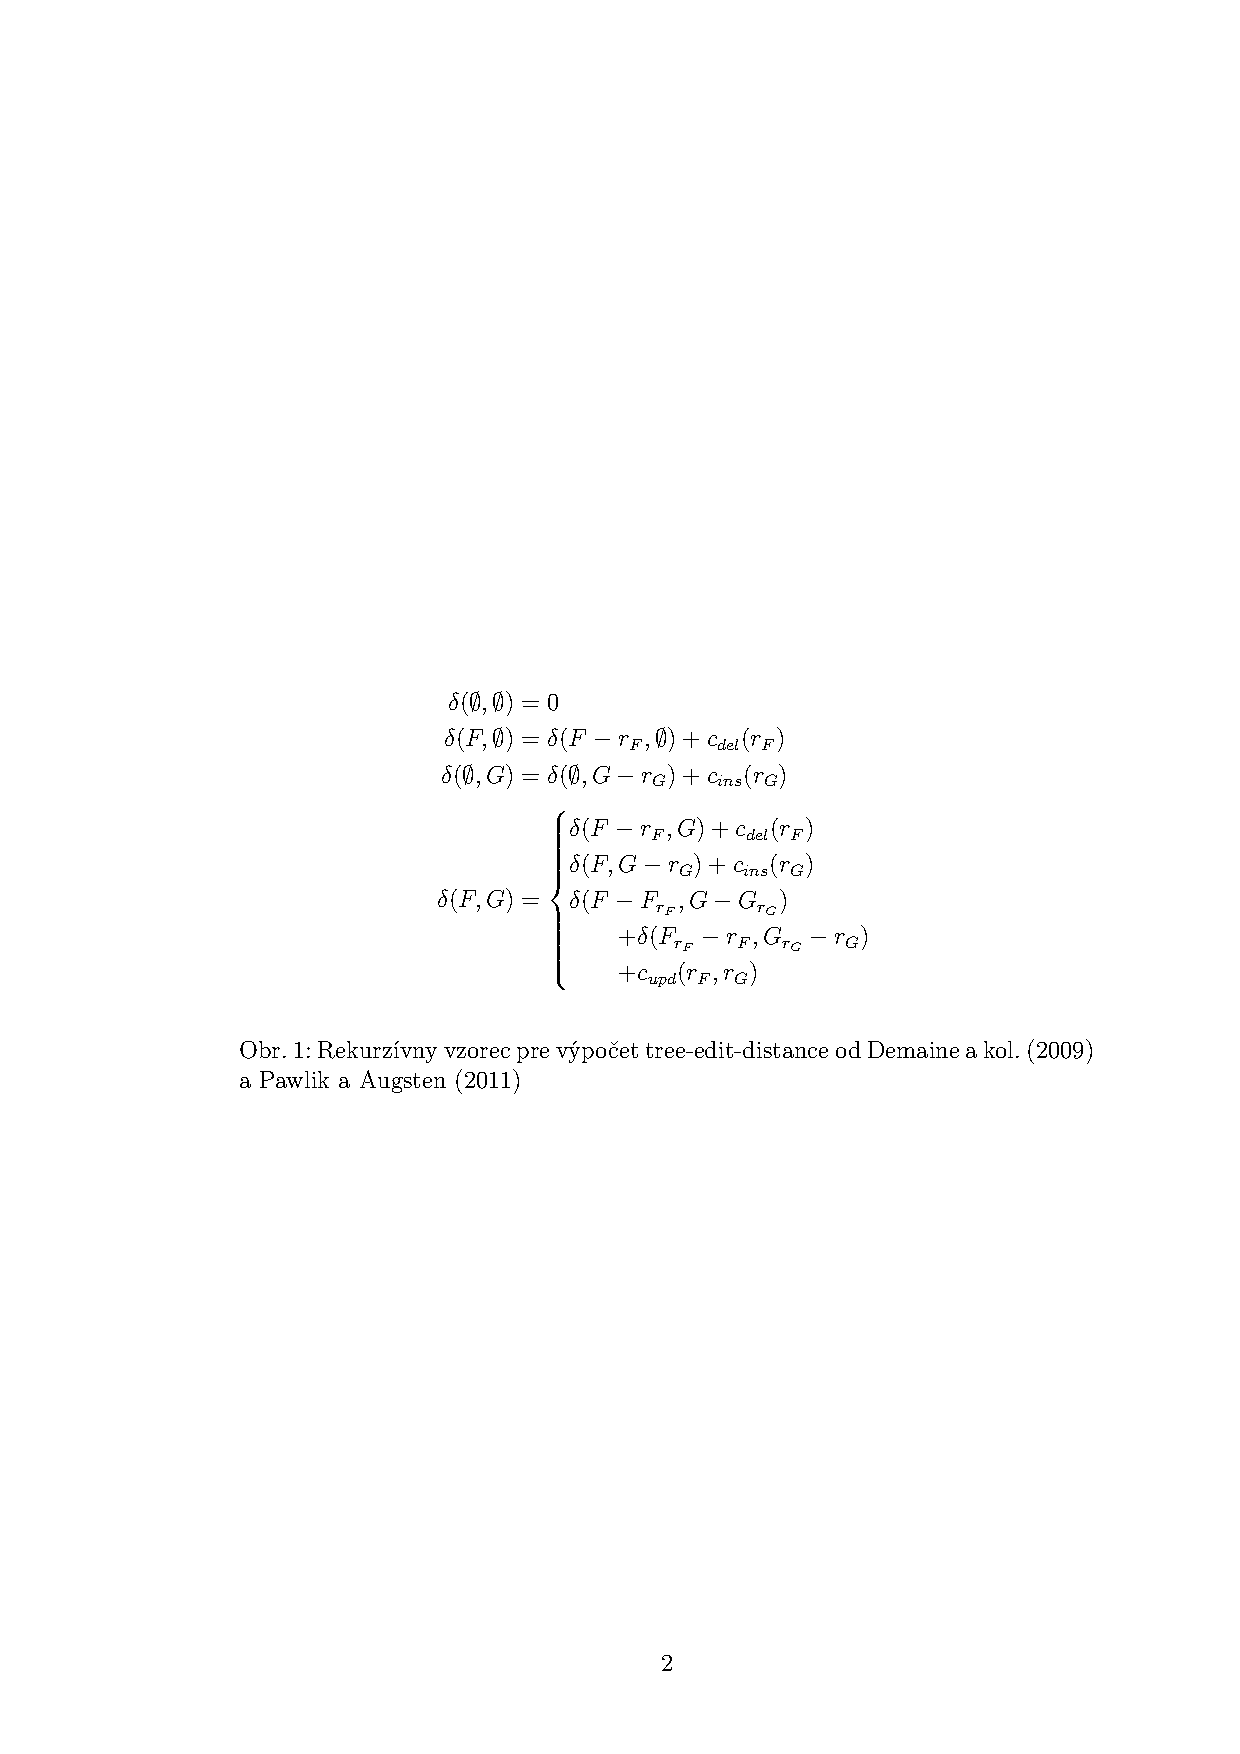
\includegraphics[clip, trim = 7cm 12.5cm 6cm 11cm, width=0.3\textwidth]{./include/ted}
          };
      \end{tikzpicture}
    \end{wrapfigure}

    Vďaka zanedbaniu existencie pseudouzlov, môžeme sekundárnu štruktúru reprezentovať
    ako usporiadaný zakorenený strom (pseudouzly sú páry vedúce medzi vetvami stromu).
    Transformácia sekundárnej štruktúry do stromovej podoby je na obrázku.
    Vnútorný vrchol stromu reprezentuje bázový pár a listy nespárované nukleotidy.

    Pôvodným nakreslením chceme hýbať čo najmenej a tak potrebujeme spôsob ako
    odlíšiť časti, ktoré sa v oboch molekulách nemenia. K tomu využijeme algoritmus
    \textit{tree-edit-distance}, ktorý nám dá návod ako určiť najmenší počet úprav,
    ktorými vieme transformovať šablónovú molekulu na cieľovú.
    Úpravami myslíme editačné operácie update, insert a delete (zmena bázy vo vrchole,
    vloženie lebo zmazanie vrcholu).

    Základom algoritmu je rekurzívny vzorec, ktorý určí vzdialenosť medzi dvoma stromami
    ($r$ označuje najpravejší, alebo najľavejší vrchol lesa $F$ a $G$,
    \Cdel, \Cins, \Cupd sú ceny mazania, vkladania a updatu vrcholu v strome).

    \vspace{5cm}
    .. tu bude este nieco pokracovat

  }
  \blocknode{Nástroj TRAVeLer}{XYZ}
  \blocknode{Výsledky}{Tu budu zhrnute vysaledky prace}
\end{tikzpicture}
\end{document}
